\documentclass[a4paper,11pt,final]{article}
% Pour une impression recto verso, utilisez plutôt ce documentclass :
%\documentclass[a4paper,11pt,twoside,final]{article}

\usepackage[english,francais]{babel}
\usepackage[utf8]{inputenc}
\usepackage[T1]{fontenc}
\usepackage[pdftex]{graphicx}
\usepackage{setspace}
\usepackage{hyperref}
\usepackage[french]{varioref}

\newcommand{\reporttitle}{Exemple de rapport}     % Titre
\newcommand{\reportauthor}{Bruno \textsc{Voisin}} % Auteur
\newcommand{\reportsubject}{Stage de fin d'étude} % Sujet
\newcommand{\HRule}{\rule{\linewidth}{0.5mm}}
\setlength{\parskip}{1ex} % Espace entre les paragraphes

\hypersetup{
    pdftitle={\reporttitle},%
    pdfauthor={\reportauthor},%
    pdfsubject={\reportsubject},%
    pdfkeywords={rapport} {vos} {mots} {clés}
}

\begin{document}
  % Inspiré de http://en.wikibooks.org/wiki/LaTeX/Title_Creation

\begin{titlepage}

\begin{center}

\begin{minipage}[t]{0.48\textwidth}
  \begin{flushleft}
    
\includegraphics [width=30mm]{images/logo-univ.jpg} \\[0.5cm]
    \begin{spacing}{1.5}
      \textsc{\LARGE Université de ...}
    \end{spacing}
  \end{flushleft}
\end{minipage}
\begin{minipage}[t]{0.48\textwidth}
  \begin{flushright}
    
\includegraphics [width=30mm]{images/logo-societe.jpg} \\[0.5cm]
    \textsc{\LARGE Entreprise}
  \end{flushright}
\end{minipage} \\[1.5cm]

\textsc{\Large \reportsubject}\\[0.5cm]
\HRule \\[0.4cm]
{\huge \bfseries \reporttitle}\\[0.4cm]
\HRule \\[1.5cm]

\begin{minipage}[t]{0.3\textwidth}
  \begin{flushleft} \large
    \emph{Auteur :}\\
    \reportauthor
  \end{flushleft}
\end{minipage}
\begin{minipage}[t]{0.6\textwidth}
  \begin{flushright} \large
    \emph{Responsables :} \\
    M.~Jean \textsc{Machin} \\
    M.~Pierre \textsc{Bidon}
  \end{flushright}
\end{minipage}

\vfill

{\large 17 novembre 2011}

\end{center}

\end{titlepage}

  \cleardoublepage % Dans le cas du recto verso, ajoute une page blanche si besoin
  \tableofcontents % Table des matières
  \sloppy          % Justification moins stricte : des mots ne dépasseront pas des paragraphes
  \cleardoublepage
  \section*{Remerciements}
\addcontentsline{toc}{section}{Remerciements}

Je tiens à remercier \LaTeX{} et les tutoriels sur internet et notamment \url{http://www.ukonline.be/programmation/latex/tutoriel/index.php}.

Bla bla bla bla bla.

  \cleardoublepage
  \section*{Introduction} % Pas de numérotation
\addcontentsline{toc}{section}{Introduction} % Ajout dans la table des matières

Ce document est un exemple de rapport. J'espère aider des étudiants à réaliser leur rapport en \LaTeX.

Écrit par Bruno Voisin (Hiko Sejûrô) et publié sur \url{http://blog.hikoweb.net/}.

  \cleardoublepage
  \section{La première section}


\subsection{Une sous section}

On peut mettre des mots en \emph{italique}, 
en \textsc{petites Majuscules} ou 
en \texttt{largeur fixe (machine à écrire)}.

Voici un deuxième paragraphe avec une formule mathématique simple : $e = mc^2$.

Un troisième avec des \og guillemet français \fg{}.

\subsubsection{Écrire en anglais}

\foreignlanguage{english}{Do you speak French? Does anybody here speak french?}


\subsection{Lites}

\begin{itemize}
\item Liste classique ;
\item un élément ;
\item et un autre élément.
\end{itemize}
\vspace{\parskip} % espace entre paragraphes

\begin{enumerate}
\item Une liste numéroté
\item deux
\item trois
\end{enumerate}
\vspace{\parskip}

\begin{description}
\item[Description] C'est bien pour des définitions.
\item[Deux] Ou pour faire un liste spéciale.
\end{description}
\vspace{\parskip}


\subsection{Références}

Voici une référence à l'image de la figure \ref{bloghiko} page \pageref{bloghiko} et une autre vers la partie \ref{p2} page \pageref{p2}.

On peut citer un livre\,\up{\cite{lpp}} et on précise les détails à la fin du rapport dans la partie références.


\subsection{Note de bas de page}

Voici une note\,\footnote{Texte de bas de page} de bas de page.
Une deuxième\,\footnotemark{} déclarée différemment.
La même note\,\footnotemark[\value{footnote}].

\footnotetext{Il a deux références vers cette note}


\subsection{Figure}

\begin{figure}[!ht]
    \center
    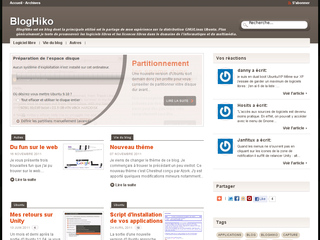
\includegraphics[]{./images/bloghiko.jpg}
    \caption{BlogHiko | taille original}
    \label{bloghiko}
\end{figure}

\begin{figure}[!ht]
    \center
    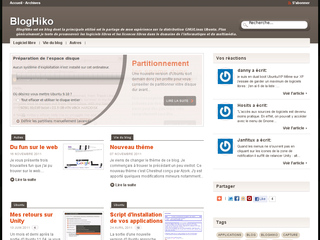
\includegraphics[width=0.5\textwidth]{./images/bloghiko.jpg}
    \caption{BlogHiko | 50\% de la largeur de la page}
\end{figure}



  \cleardoublepage
  \section{Citation Wikipédia}
\label{p2}


LaTeX est un langage et un système de composition de documents créé par Leslie Lamport en 198312. Plus exactement, il s'agit d'une collection de macro-commandes destinées à faciliter l'utilisation du \og processeur de texte \fg{} TeX de Donald Knuth. Depuis 1993, il est maintenu par le LaTeX3 Project team. La première version utilisée largement, appelée LaTeX2.09, est sortie en 1984. Une révision majeure, appelée LaTeX2 epsilon est sortie en 1991.

Le nom est l'abréviation de Lamport TeX. On écrit souvent \LaTeX, le logiciel permettant les mises en forme correspondant au logo.

Du fait de sa relative simplicité, il est devenu la méthode privilégiée d'écriture de documents scientifiques employant TeX. Il est particulièrement utilisé dans les domaines techniques et scientifiques pour la production de documents de taille moyenne ou importante (thèse ou livre, par exemple). Néanmoins, il peut aussi être employé pour générer des documents de types variés (par exemple, des lettres, ou des transparents).


  \cleardoublepage
  \section*{Conclusion}
\addcontentsline{toc}{section}{Conclusion}

Pour conclure, avec \LaTeX{} on obtient un rendu impeccable mais il faut s'investir pour le prendre en main.

  \cleardoublepage
  \phantomsection\addcontentsline{toc}{section}{Références}
\begin{thebibliography}{ABC}	
    \bibitem[REF]{reference} auteur. \emph{titre}. édition, année.
    \bibitem[LPP]{lpp} Rolland. \emph{LaTeX par la pratique}. O'Reilly, 1999.
\end{thebibliography}

\end{document}

